\dummypart{2}{Polynomials}
\myLesson{Synthetic Division}[11]

\begin{myObjectives}
    \myObjective{divide}{two polynomials by \gap{synthetic} \gap{division}}
    \myObjective{determine}{if a binomial is a factor using \gap{synthetic} \gap{division}}
\end{myObjectives}

\begin{myVocabulary}
    \myDefinition{dividend}{the \gap{numerator} when you divide}
    \myDefinition{divisor}{the \gap{denominator} when you divide}
    \myDefinition{quotient}{the \gap{main} \gap{result} of division}
    \myDefinition{remainder}{what is \gap{left} \gap{over}}
    \myDefinition{synthetic}{imitation, for \gap{special} situations}
    \myDefinition{descending order}{starting with the \gap{largest} exponent and going down}
    \myDefinition{coefficient}{the number in front of a variable}
\end{myVocabulary}

All these things are \gap{closely} \gap{related}.
Given one, you can \gap{find} \gap{the} \gap{others}.

\begin{center}  
    \small  
    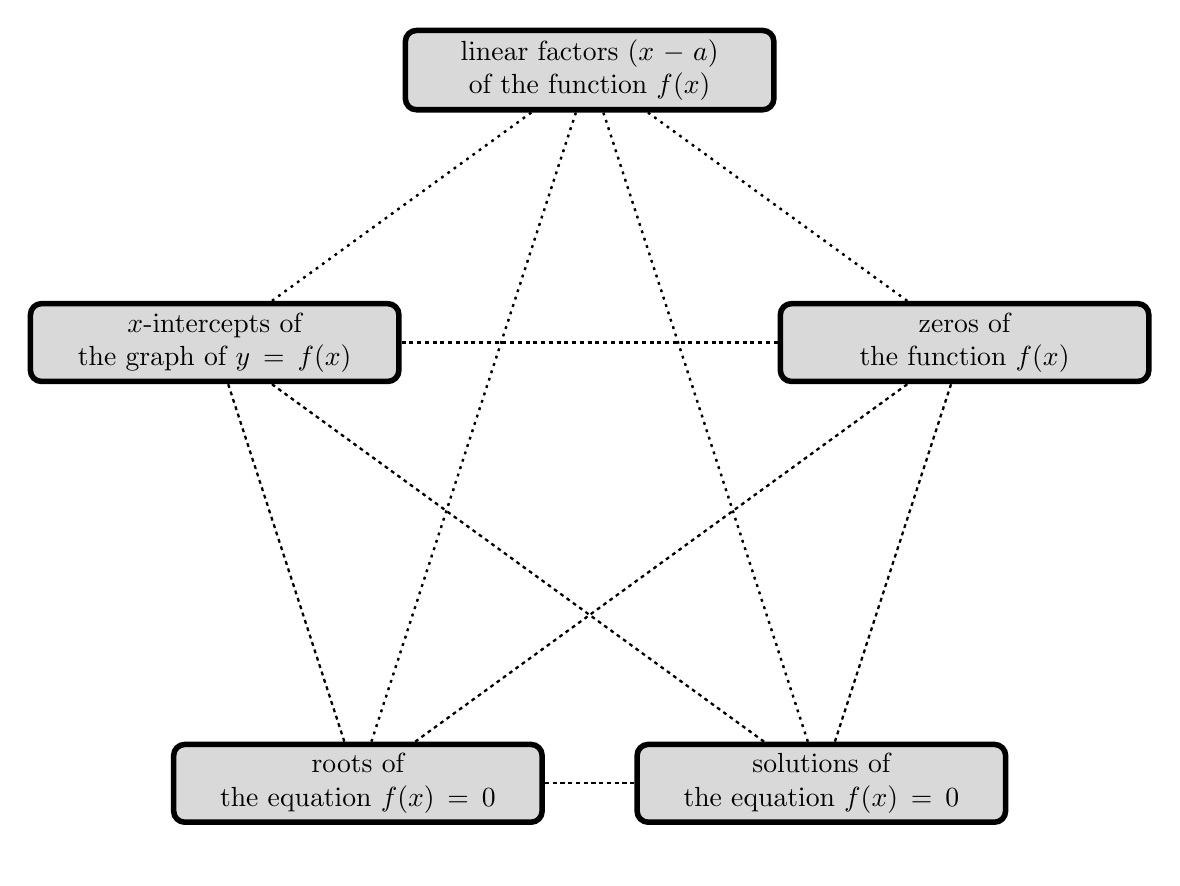
\begin{tikzpicture}
        % Draw a circle around which I'll place nodes.
        \node[circle,minimum size=10cm] (Z) {};
        %
        % Place 5 nodes around the circle.
        \node (rect) [draw,text width=1.75in, align=center,line width=2pt,rounded corners=4pt,fill=black!15] 
            (n-1) at (Z.{90})
            {
                \myEmph{linear factors} $(x-a)$\linebreak
                of the function $f(x)$
            };
        \node (rect) [draw,text width=1.75in, align=center,line width=2pt,rounded corners=4pt,fill=black!15] 
            (n-2) at (Z.{90+72})
            {
                \myEmph{$x$-intercepts} of\linebreak
                the graph of $y=f(x)$
            };
        \node (rect) [draw,text width=1.75in, align=center,line width=2pt,rounded corners=4pt,fill=black!15] 
            (n-3) at (Z.{90+144})
            {
                \myEmph{roots} of\linebreak
                the equation $f(x)=0$
            };
        \node (rect) [draw,text width=1.75in, align=center,line width=2pt,rounded corners=4pt,fill=black!15] 
            (n-4) at (Z.{90+216})
            {
                \myEmph{solutions} of\linebreak
                the equation $f(x)=0$
            };
        \node (rect) [draw,text width=1.75in, align=center,line width=2pt,rounded corners=4pt,fill=black!15] 
            (n-5) at (Z.{90+288})
            {
                \myEmph{zeros} of\linebreak
                the function $f(x)$
            };
        %
        % Connect all the nodes by lines.
        \foreach\x in{1,...,5}{
            \foreach\y in{1,...,5}{
            \ifnum\x=\y\relax\else
                \draw (n-\x) edge[-,dotted,thick] (n-\y);
            \fi
            }
        }
    \end{tikzpicture}
\end{center}
% \section{Quick Polynomial Division Using Synethetic Division}

% % \begin{myCenteredBox}[width=5.25in,]
%     \gap{Synthetic} division is an alternative to \gap{long} division.
%     Use it when the {\bfseries\itshape divisor} is a \gap{linear} \gap{binomial}. 
%     \begin{itemize}[nosep]
%         \item It is fast.
%         \item It is short.
%     \end{itemize}
% % \end{myCenteredBox}


\begin{myConceptSteps}{~To divide polynomials using synthetic division\dots}
    \myStep{setup}{%
        \begin{itemize}[nosep,leftmargin=*]
            \item Draw an L-shaped frame for two rows of numbers.
            \item Write the coefficients of the {\bfseries\scshape Dividend}.
                \begin{itemize}[nosep,leftmargin=*]
                    \item[$\circ$] in \gap{descending} exponent order
                    \item[$\circ$] with \gap{zeros} for missing terms
                \end{itemize}
            \item Write $a$ from the {\bfseries\scshape Divisor}. 
                \begin{itemize}[nosep,leftmargin=*]
                    \item[$\circ$] $a$ is the \gap{opposite} of what you see.
                \end{itemize}
        \end{itemize}
    }
    \myStep{start}{Bring the \gap{leading} coefficient down.}
    \myStep{multiply}{Multiply $a$ times the number at the bottom.}
        \begin{itemize}[nosep,leftmargin=*]
            \item Put it under the next coefficient.
        \end{itemize} 
    \myStep{add}{Add the numbers in the right column.}
        \begin{itemize}[nosep,leftmargin=*]
            \item Put the sum at the bottom.
        \end{itemize} 
    \myStep{repeat}{Repeat until done. (Goto step 3.)}
    \myStep{identify}{Identify the {\bfseries\scshape Quotient} and {\bfseries\scshape Remainder}.}
    \myStep{result}{%
        The result is 
        {
            $ 
                \text{\bfseries\scshape Quotient} 
                + 
                \frac{\text{\bfseries\scshape Remainder}}{\text{\bfseries\scshape Divisor}} 
            $
        }
    }
\end{myConceptSteps}

\myProblems[Divide these polynomials.]
    {
        $
            (x^3 + 18x^2 + 71x -74) 
            \div
            (x+8)
        $
    }
    {
        \Large
        $\frac
            {t^3 - 49t -8} 
            {t - 7}
        $
    }
    {2.5in}

\begin{myConceptSteps}{
    To solve a \gap{quadratic} equation using the quadratic formula\dots
}
\myStep{standard form}{Write the equation as \gap{$ax^2 + bx + c = 0$}.}
\myStep{coefficients}{Write down the values of \gap{$a$}, \gap{$b$}, \gap{$c$}. }
\myStep{discriminant}{Calculate the discriminant as \gap{$ D = b^2 - 4ac $}.}
\myStep{quadratic formula}{
    The quadratic formula is:
    \begin{tcolorbox}[center,width=1.5in,colback=white,]
        $\displaystyle x = \frac{-b \pm \sqrt{D}}{2a}$
    \end{tcolorbox}
    {\normalsize 
    which is really \gap{two} solutions:
    \begin{align*} 
        x &= \frac 
        {-b \bm{+} \myRoot{b^2 - 4ac}}
        {2a}
        &
        x &= \frac 
        {-b \bm{-} \myRoot{b^2 - 4ac}}
        {2a}
    \end{align*}
    }
}
\myStep{substitute}{Substitute $a$, $b$, $c$, and $D$ into this formula.
Usually you will get \gap{two} solutions.
\begin{itemize}
    \item When $D =$ \gap{$0$}, there is only \gap{one} \gap{solution}.
    \item When $D$ is \gap{negative}, there are \gap{no} \gap{real} \gap{solutions}.
\end{itemize}
}
\myStep{evaluate}{\gap{Simplify} the right-hand-side of the equations.}
\end{myConceptSteps}
